\subsection{Circuito Driver}

Como se explicó más arriba, para excitar un transistor MOSFET y encenderlo, es necesario mantener una tensión $V_{GS}$ entre gate y source mayor a una tensión umbral dependiente del modelo. En nuestro caso, esta tensión umbral del IRFP150N es de \SI[]{4}[]{\volt}, como se ve en la tabla \ref{tabla:IRFP150}. Entonces, se debe diseñar algún circuito que sea capaz de proveer estos pulsos de tensión al gate de cada transistor, entregando también la corriente necesaria para cargar y descargar sus capacitancias de gate suficientemente rápido (llamadas corrientes de \textit{source} y \textit{sink}).\\

Este es el llamado {\Medium circuito \textit{driver}} o {\Medium circuito de excitación} y debe existir uno para cada uno de los cuatro transistores del puente. Ahora debemos establecer algunos requerimientos que debe cumplir el circuito:\\

\begin{itemize}
    \item Tensión de operación mayor a \SI[]{100}[]{\volt}, por encima de la máxima tensión de la pila de combustible.
    \item Tiempos de encendido y apagado mucho menores al período $T_s$ de \SI[]{50}[]{\micro\second} de la excitación.
    \item Corrientes de sink y source mayores a \SI[]{2}[]{\ampere} para cargar rápidamente las capacitancias de los transistores, calculado según la nota de aplicación de \cite{SinkSourceCurrent}.
    \item Se busca utilizar una solución integrada, ya que suelen ser más compactas y sencillas.
    \item Es deseable el uso de componentes de montaje superficial o SMD.\\
\end{itemize}

Con estos datos vamos a seleccionar y diseñar un circuito de excitación y explicar brevemente el funcionamiento de todas sus partes.\\

\subsubsection{Selección del Integrado}

Existen diversos tipos de soluciones integradas para circuitos de excitación de transistores MOSFET. Se pueden encontrar circuitos de uno o múltiples canales; existen circuitos que incluyen una aislación entre las entradas y salidas; entre otras funcionalidades. También se consiguen con distintas funciones de seguridad y protección, como el \textit{dead-time}, que permite forzar un tiempo fijo entre la activación de dos transistores de la misma rama, evitando situaciones de cortocircuito; y el \textit{undervoltage lockout} (UVLO), que evita daños por condiciones de baja tensión.\\

Entre todas las opciones, originalmente se había decidido por el modelo UCC21540 de Texas Instruments, un driver de doble canal, con aislación incluida, funcionalidades de dead-time y UVLO, alta capacidad de corriente y un encapsulado SMD de tipo SOIC-16.\\

Sin embargo, este dispositivo no se pudo obtener por falta de disponibilidad, por lo que se tuvo que buscar una alternativa de características similares que esté en disponibilidad. Se terminó decidiendo por el integrado {\Medium 2ED21834-S06J de Infineon Technologies}, cuyas especificaciones básicas se muestran en la tabla \ref{tabla:driver}.\\

\setlength{\tabcolsep}{7pt}
\renewcommand{\arraystretch}{1.5}
\begin{table}[h]
\begin{center}
    \begin{tabular}{llrrrr}
    {\SemiBold Fabricante} & {\SemiBold Modelo} & $\mathbf{V_S}$ [\unit{\volt}] & $\mathbf{I_{OH}/\mathbf{I_{OL}}}$ [\unit{\ampere}] & $\mathbf{t_{on}}/\mathbf{t_{off}}$ [\unit{\nano\second}] & $\mathbf{V_{cc}}$ [\unit{\volt}]\\
    \hline
    \makecell[l]{Infineon \\ Technologies} & 2ED21834-S06J & \num{650} & \num{2.5} & \num{200} & \num{10}-\num{20}
    \end{tabular}
    \caption{Especificaciones del driver modelo 2ED21834-S06J de Infineon Technologies.\textsuperscript{\cite{DatasheetDriver}}}
    \label{tabla:driver}
\end{center}
\end{table}

Donde $V_S$ es la máxima tensión común de operación, $I_{OH}$ e $I_{OL}$ son las corrientes máximas de source y sink, $t_{on}$ y $t_{off}$ son los tiempos de encendido y apagado, y $V_{cc}$ es el rango de tensiones de alimentación.\\ 

El 2ED21834-S06J es un driver de doble canal para medios puentes de transistores de tipo MOSFET e IGBT, con diodo y resistencia de bootstrap incluidos además de funcionalidad de dead-time y UVLO para circuitos del lado bajo y alto, todo contenido en un encapsulado SMD de catorce pines del tipo DSO-14 (figura \ref{encapsulado_driver}). Sus corrientes sink y source de \SI[]{2.5}[]{\ampere} superan la corriente necesaria calculada para los IRFP150N de la tabla \ref{tabla:IRFP150}, su tensión de operación se encuentra cómodamente por encima de la tensión de operación del primario del convertidor, además de tener muy bajos tiempos de conmutación.\\

\begin{figure}[h]
    \centering
    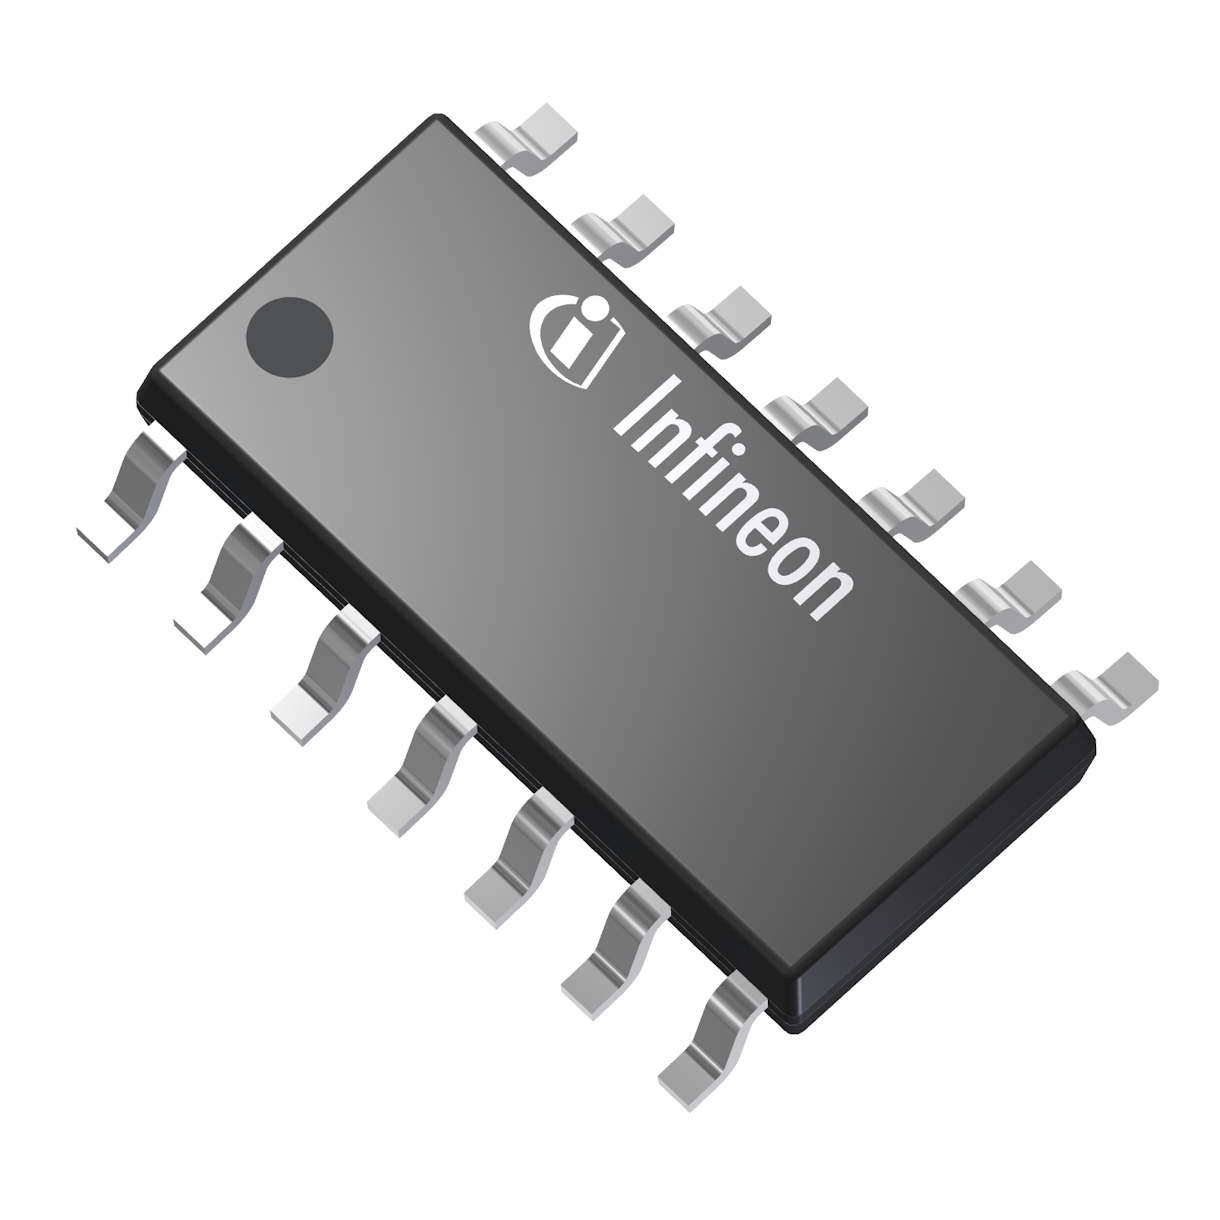
\includegraphics[scale=0.07]{Imagenes/Driver DSO-14.png}
    \caption{Driver 2ED21834-S06J con su encapsulado SMD tipo DSO-14.}
    \label{encapsulado_driver}
\end{figure}

En nuestro caso, se deben utilizar dos de estos dispositivos, uno para cada columna del puente completo. Vamos a utilizar la función de dead-time, configurable mediante una resistencia conectada al pin DT, para proteger contra posibles cortocircuitos causados por la activación errónea de ambos transistores de una columna simultáneamente (\textit{shoot-through}). El resto de la conexión de componentes del driver se realizó de acuerdo a las recomendaciones del fabricante encontradas en la hoja de datos \cite{DatasheetDriver}, que se puede ver en la figura \ref{circuito_driver}.\\

\begin{figure}[h]
    \centering
    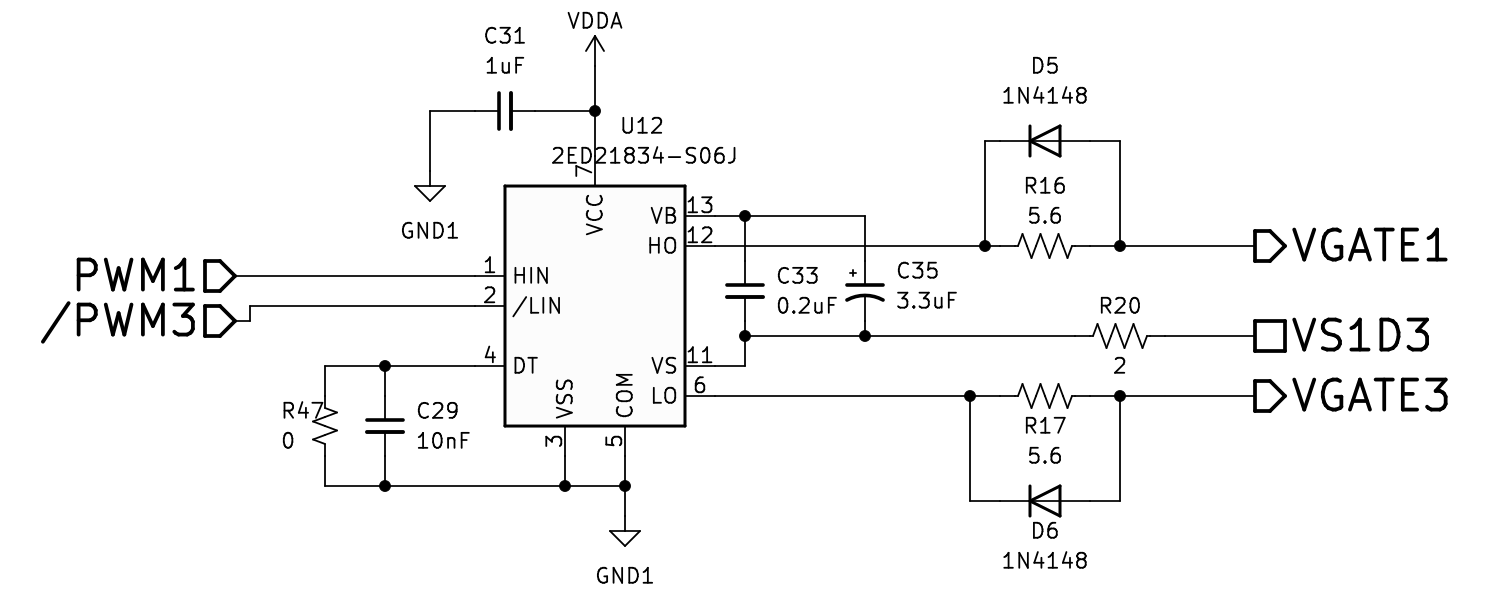
\includegraphics[scale=0.95]{Imagenes/Circuito Driver.png}
    \caption{Circuito de conexión del driver 2ED21834-S06J. El circuito del driver para la otra columna es idéntico.}
    \label{circuito_driver}
\end{figure}

Aquí se puede ver el driver, indicado por la referencia U12, al que le llegan las señales de comando PWM a sus pines HIN y /LIN para el transistor del lado alto y bajo de la columna respectivamente (al estar negada  la entrada para el transistor bajo, la señal que le llega debe estar invertida). Luego, conectado entre el pin DT y tierra se encuentra la resistencia de dead-time, que cuyo valor define el dead-time o tiempo muerto $t_{DT}$. En la salida, se conecta a los pines HO (alto) y LO (bajo) una resistencia limitadora en paralelo con un diodo que permite la descarga de las capacitancias de los transistores, y entre los pines VB y VS se coloca el capacitor que completa el circuito de bootstrap, que se explicará mas adelante. En lo que hace referencia a conexiones a tierra, este circuito, al estar del lado primario del convertidor, se conecta a la referencia $GND_1$. Según la hoja de datos, la tensión de alimentación debe ser de entre \SI[]{10}[]{\volt} y \SI[]{20}[]{\volt}, por lo que se alimenta con una tensión no regulada de \num{12}-\SI[]{18}[]{\volt}.\\

El dimensionamiento de todos estos componentes se va a tratar a continuación siguiendo las recomendaciones del fabricante disponibles en hojas de datos y notas de aplicación.\\

\subsubsection{Dimensionamiento de Componentes}

\paragraph{Resistencia de Dead-Time (R47)}

La resistencia de dead-time $R_{DT}$, con el identificador R47 en el diagrama circuital de la figura, es una resistencia conectada entre el pin DT y tierra, cuya funcionalidad es configurar la duración del dead-time $t_{DT}$ entre los disparos del transistor superior e inferior conectados al driver. El dead-time es un pequeño intervalo de tiempo luego de la desactivación de cada llave, en el cual el integrado no permite que se dispare el otro transistor, con el objetivo de no permitir la activación accidental de ambos transistores y evitar cortocircuitar la pila de combustible.\\

\begin{figure}[h]
    \centering
    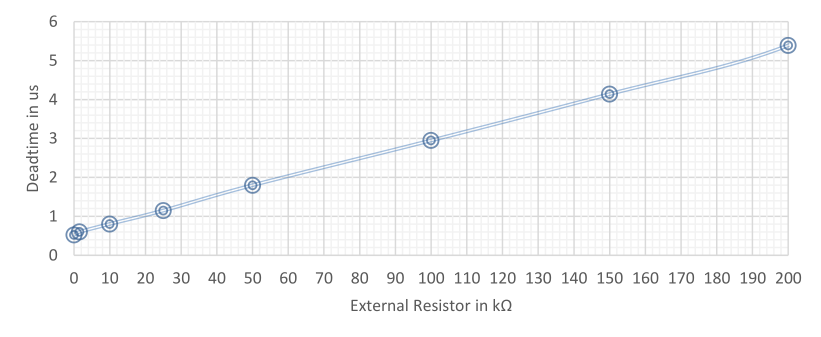
\includegraphics[scale=0.5]{Imagenes/Curva Dead-Time.png}
    \caption{Curva de dead-time contra resistencia para el integrado 2ED21834-S06J.\textsuperscript{\cite{DatasheetDriver}}}
    \label{curva_deadtime}
\end{figure}

En la figura \ref{curva_deadtime} se presenta la curva que relaciona el dead-time $t_{DT}$ con el valor de la resistencia $R_{DT}$, dónde se puede ver que existe una relación altamente lineal, variando entre un tiempo de \SI{400}{\nano\second} para \SI[]{0}{\ohm} de resistencia y \SI[]{5}{\micro\second} para \SI[]{200}{\kilo\ohm}.\\

La duración de $t_{DT}$ debe ser seleccionada de manera de ser cómodamente mayor al tiempo de apagado $t_{on}$ de los transistores, de \SI[]{85}{\nano\second} para los IRFP150 (tabla \ref{tabla:IRFP150}). Al mismo tiempo, también debe ser mucho menor a la duración de un semiciclo de las señal PWM de excitación, cuya duración es de \SI[]{25}{\micro\second}. Por esta razón, se eligió {\Medium cortocircuitar el pin DT a tierra} (colocar una resistencia de \SI[]{0}{\ohm}), obteniendo un {\Medium dead-time de 400 ns}, que es cinco veces mayor al tiempo de apagado de un IRFP150 y más de 60 veces más corto que un semiciclo de la señal de excitación.\\

Finalmente, en paralelo con $R_{DT}$ se colocó un capacitor cerámico $C_{DT}$ (C29 en la figura \ref{circuito_driver}) de desacople de \SI[]{10}{\nano\farad}, de acuerdo a la recomendación del fabricante de colocar un capacitor de valor mayor a \SI[]{1}{\nano\farad}.\\

\paragraph{Circuito Bootstrap}

El circuito de bootstrap es un circuito compuesto por tres elementos en serie: un capacitor de bootstrap $C_{BS}$, un diodo de bootstrap $D_{BS}$ y una resistencia de bootstrap $R_{BS}$. En el caso del circuito del dirver de la figura \ref{circuito_driver}, se pueden ver los capacitores C33 y C35 que conforman la capacidad $C_{BS}$, mientras que la resistencia y el diodo se encuentran integrados dentro de 2ED21834-S06J, como se observa en la figura \ref{circuito_bootstrap}, tomada de la hoja de datos del integrado.\\

\begin{figure}[h]
    \centering
    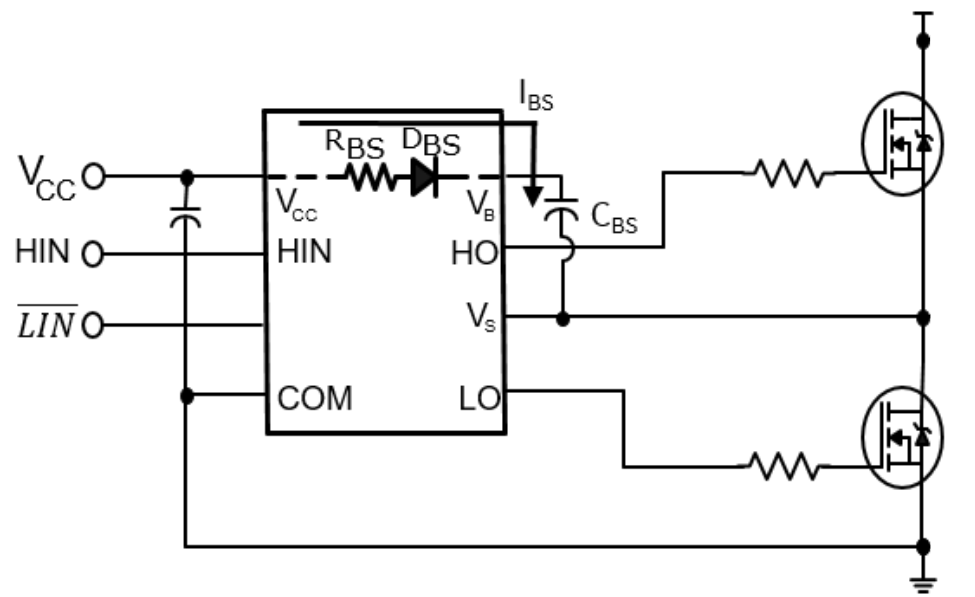
\includegraphics[scale=1]{Imagenes/Circuito Bootstrap.png}
    \caption{Circuito bootstrap con diodo y resistencia serie internos del 2ED21834-S06J.\textsuperscript{\cite{DatasheetDriver}}}
    \label{circuito_bootstrap}
\end{figure}

Este circuito se utiliza en drivers para configuraciones de medio puente, con la funcionalidad de proveer la polarización necesaria para poder disparar el MOSFET del lado alto. Cuando el MOSFET del lado bajo se encuentra encendido (y por lo tanto el MOSFET del lado alto apagado), el pin VS se conecta a tierra y circula una corriente a través del diodo $D_{BS}$ y resistencia $R_{BS}$ que carga el capacitor de bootstrap externo $C_{BS}$. Cuando la situación se invierte, con el MOSFET superior encendido y el inferior apagado, el pin VS se conecta a la tensión superior, y $C_{BS}$ descarga su tensión acumulada durante la fase previa sobre la compuerta del MOSFET superior mediante el pin HO.\\

Entonces, solo hace falta dimensionar el capacitor $C_{BS}$, ya que tanto la resistencia como el diodo se encuentran integrados dentro del dispositivo y no es posible ajustar sus valores. Como una regla general, este capacitor debe almacenar una cantidad de carga lo suficientemente grande como para no perder más del 10\% de su carga durante el disparo y activación del MOSFET superior, o también, su capacidad debe ser al menos 10 veces mayor que la capacidad de gate $C_g$ del MOSFET a disparar.\textsuperscript{\cite{Bootstrap}}

\begin{equation*}
    C_{BS} \gg C_g
\end{equation*}

Esta capacidad de gate se puede calcular en base a la carga de gate total $Q_g$, que se puede encontrar en la hoja de datos del IRFP150 con un valor de \SI[]{110}{\nano\coulomb}.

\begin{equation}\label{capacidad_gate}
    C_g = \frac{Q_g}{V_{cc}-V_{D_{BS}}} = \frac{\SI[]{110}{\nano\coulomb}}{\SI[]{12}{\volt}-\SI[]{1.2}{\volt}} \approx \SI[]{10}{\nano\farad}
\end{equation}

Por lo tanto, la cota mínima del capacitor de bootstrap resulta:

\begin{equation}\label{capacidad_bs_min}
    \boxed{\highlight{
    C_{BS} > \SI[]{0.1}{\micro\farad} = 10\cdot C_g}}
\end{equation}

Como este valor es muy pequeño, y la hoja de datos del driver indica que se pueden utilizar capacidades $C_{BS}$ de hasta \SI[]{4.7}{\micro\farad}, se decidió utilizar un capacitor electrolítico de montaje through-hole, \SI[]{3.3}{\micro\farad} de capacidad y tensión máxima de \SI[]{50}{\volt}. Adicionalmente, según recomendación del fabricante, se agregó un capacitor cerámico de mucho menor valor (C33 en el circuito) en paralelo a $C_{BS}$ para obtener una solución óptima.\\

\paragraph{Resistencia de VS}

La resistencia colocada en serie al pin VS, identificador R20 en el diagrama de la figura \ref{circuito_driver}, según la hoja de datos del fabricante, cumple el objetivo de reducir los picos negativos de tensión al momento de la conmutación, inducidos en VS por elementos parásitos de la placa de circuito impreso. Se indica que esta debe ser una resistencia con un valor máximo de \SI[]{5}{\ohm}\textsuperscript{\cite{DatasheetDriver}}, por lo que se decidió por colocar un pequeño resistor SMD 1206 de \SI[]{2}{\ohm}.\\